% Master File: usersmanual.tex
% Document Type: PDFLaTeX
\documentclass[english]{report}
\usepackage[T1]{fontenc}
\usepackage[utf8]{inputenc}
\usepackage{fullpage}
\setcounter{secnumdepth}{3}
\setcounter{tocdepth}{4}
\usepackage{babel}
\usepackage{amsmath}
\usepackage{amssymb}
\usepackage{graphicx}
\usepackage{cite}
\usepackage{color} 
\usepackage{comment}
\usepackage{url}
\usepackage{hyperref}
\usepackage{verbatim}

\begin{document}
\title{\textsc{TXTL matlab toolbox - User's manual}}
\date{\textsc{version 1.0}}
\author{\textsc{Zoltan A. Tuza, Vipul Singhal, Richard M. Murray}}
\maketitle
\textsc{\tableofcontents}

% Master File: usersmanual.tex
%!TEX root = usersmanual.tex
\chapter{\textsc{The TXTL Modelling Toolbox}}

The TXTL modelling toolbox for MATLAB is a companion to the TXTL Breadboards (Cell-free expression) project being developed at the California Institute of Technology and the University of Minnesota. This toolbox aims to allow \textit{in-silico} prototyping of circuits before they are built \textit{in-vitro}, and to provide insight into circuit behaviour. 

\section{Protocol Overview}

The cell-free circuit breadboard family is a collection of in vitro
protocols that can be used to test transcription and translation
(TX-TL) circuits in a set of systematically-constructed environments
that explore different elements of the external conditions in which
the circuits must operate. This breadboard is based on the work of
Vincent Noireaux at U. Minnesota. The transcription and translation
machineries are extracted from E. coli cells (Shin and Noireaux,
2010). The endogenous DNA and mRNA from the cells are eliminated
during the preparation. The resulting protein synthesis machinery is
used to program cell-free TX-TL gene circuits in reactions of
12uL. The gene circuits can engineered in the laboratory using
standard molecular cloning techniques, but it is also possible to use
PCR products (linear DNA), which substantially decreases the design
cycle time. 

\begin{comment}
\subsection{The TXTL Experimental Protocol}

The endogenous Escherichia coli based TX-TL cell-free expression
system described here is an easy-to-run three-tube reaction that can
take less than 8 hours to set-up, collect, and interpret data. 

\subsection{The TXTL Modelling Protocol}
\end{comment}

The TXTL toolbox commands follow the experimental protocols closely,
and a sample code is given below with brief explanations
of the commands. More detailed explanations can be found in the
'Core Functionalities' chapter. More examples can be found in
the 'Examples' Directory, and are documented in the 'Examples' Chapter
below.

The following code sets up a simple simulation of a negatively
autoregulated gene in the TXTL system (\texttt{negautoreg.m} in the examples directory):
\begin{verbatim}
% Set up the standard TX-TL tubes
tube1 = txtl_extract('E9');
tube2 = txtl_buffer('E9');

% Set up a tube that will contain our DNA
tube3 = txtl_newtube('negautoreg');

dna_tetR = txtl_add_dna(tube3, 'ptet(50)', 'rbs(20)', 'tetR(1200)', 1, 'plasmid');

% Mix the contents of the individual tubes 
Mobj = txtl_combine([tube1, tube2, tube3]);
 txtl_addspecies(Mobj, 'aTc', 600);
 
% Run a simulation
simulationTime = 14*60*60;


tic
[simData] = txtl_runsim(Mobj,simulationTime);
toc
t_ode = simData.Time;
x_ode = simData.Data;

% Plot the results
txtl_plot(t_ode,x_ode,Mobj);
\end{verbatim}
Figure~\ref{fig:intro:negautoreg} shows the output from this code (plotted
using the \url{txtl_plot} function).
\begin{figure}
  \centering
  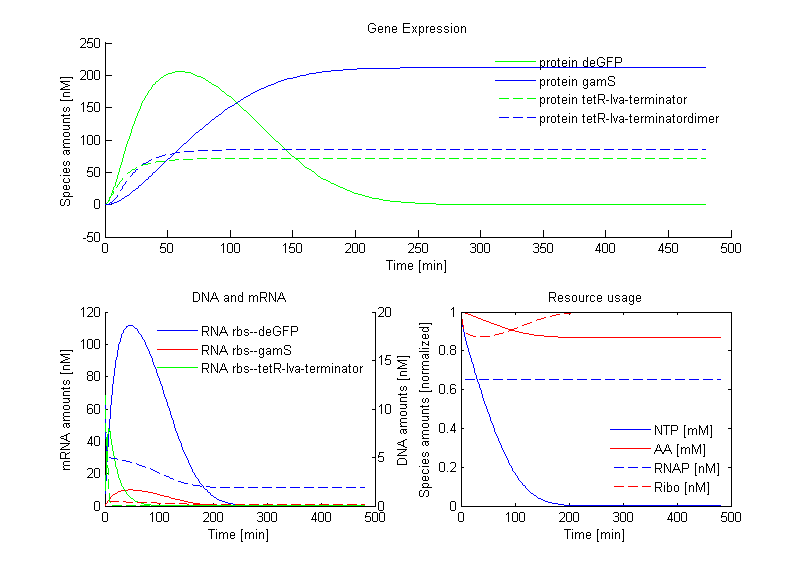
\includegraphics[width=\textwidth]{NegativeAutoregulationPlotActuallyProducedByCode.png}
  \caption{Sample simulation of a negatively autoregulated
  transcriptional circuit.}
  \label{fig:intro:negautoreg}
\end{figure}


\chapter{\textsc{Installation}}
	\section{Prerequisites}
	Our toolbox builds upon basic MATLAB\texttrademark  functionality and the Simbiology toolbox. Therefore the presence of Simbiology is essential for our TXTL toolbox to work. The toolbox was tested on MATLABb 2012 for Mac OSX, MATLAB 2010a for Linux and MATLAB 2011b Windows. 
	\section{Installing the toolbox}
	\begin{enumerate}
\item Download the toolbox zip archive \textsf{txtl-0.2a.tgz} from the project's SourceForge\texttrademark page: \url{http://sourceforge.net/p/txtl/wiki/Home/}
\item Unzip the file into a directory of your choice. In windows, this may take two unzip steps. Ultimately, you should have a folder named txtl-0.2a. 
\item Set the MATLAB working directory to the folder txtl-0.2a, or a parent folder. 
\item You may either run \begin{verbatim} txtl_init  \end{verbatim} at the
beginning of each MATLAB session or add the following directories to
your MATLAB search path, and save: \textsf{Core, Components, Examples}. 
\item All done. Try opening and running \textsf{negautoreg.m} in the \textsf{Examples} directory. If this runs without error, you have successfully installed the TXTL modelling toolbox. Congrats!
\end{enumerate}
	
% CORE FUNCTIONALITIES	

					
\chapter{\textsc{Examples}}
	\section{Gene Expression with Fluorescent Reporter (\texttt{geneexpr})}
		\subsection{Overview}
		This example shows constitutive expression of the destabilized enhanced Green Fluorescent Protein (deGFP) from a gene on a plasmid. It shows one of the simplest circuits that can be modelled with the modelling toolbox, and in doing so, illustrates its basic features. These include displaying the evolution of the expressed protein (deGFP) levels, resource usage (Amino Acids (AA) and Nucleotide Pairs (NTPs)), the evolution of the DNA and mRNA concentrations. Figure \ref{fig:geneexpr schematic} shows a schematic of this circuit. \\
		
		\begin{figure}
		\begin{center}
		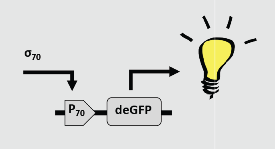
\includegraphics{geneExpr schematic.png} 
		\caption{Schematic of the gene expression circuit'}
		\label{fig:geneexpr schematic}
		\end{center}
		\end{figure}		
		 
		% show a figure with p70 promoter, rbs, DNA, leading to protein. 
		The diagram shows the DNA made of the p70 promoter, the most common constitutive promoter in the toolbox, followed by the deGFP gene. The gene is then transcribed into mRNA which is translated into DNA. 
		\ref{fig:geneexpr} shows the output plot for this example. 
		
		
		
		\subsection{Walk-through}
		If you have not already done so, ensure that you are in the \textsf{\textbackslash TXTL\_toolbox} directory, and run \texttt{txtl\_init} to add the necessary directories to the MATLAB search path. 
			
		The first step is to decide on a extract to use. The extract contains RNAP, Ribo, $\sigma 28$ and $\sigma 70$, RecBCD, RNA-ase, and sets up the reactions for the formation of RNAP70 and sequestration of RecBCD. The extract we will be using will be created using parameters defined in the external configuration file \textsf{'E6\_config.csv'}, and is implemented as: 
		
				\begin{flushleft}
						\texttt{tube1 = txtl\_extract('E6');} 
				\end{flushleft}	
				
				Note that this command returns a handle to a Simbiology model object. This is stored in the aptly named variable \texttt{tube1}. We will later combine the 'contents' of this tube with those of other tubes, just like we do in the experimental protocol. 
				
Next, we define the buffer (containing AA and NTP) to use, and store it in \texttt{tube2}. Once again, the buffer contents are drawn from the configuration file \textsf{'E6\_config.csv'}:

				\begin{flushleft}
						\texttt{tube2 = txtl\_buffer('E6');} \\	
				\end{flushleft}	 
		
We then use the \texttt{txtl\_newtube} command to create a new model object which will contain the DNA we wish to use. This is done as follows:
		
				\begin{flushleft}
						\texttt{tube3 = txtl\_newtube('circuit');} \\	
				\end{flushleft}	 
				
The next step is to define the DNA sequences to be added to \texttt{tube3}. This is done using the \texttt{txtl\_add\_dna} command:

				\begin{flushleft}
						\texttt{dna\_deGFP = txtl\_add\_dna(tube3, 'p70(50)', 'rbs(20)', 'deGFP(1000)', 4, 'plasmid');} \\	
				\end{flushleft}
Refer to the description of the \texttt{txtl\_add\_dna} command in \S 3.2 for full details of its usage. For our purposes, it suffices to now that this DNA is loaded onto a plasmid, and contains a p70 promoter (constitutive, 50 base pairs (BP) in length), a 20BP RBS domain, and a 1000BP deGFP gene. Furthermore, the DNA is such that the \textbf{final} concentration of this DNA in the \textbf{combined} tube will be 4nM. 

We then simply combine the extract, buffer, and DNA:

				\begin{flushleft}
						\texttt{Mobj = txtl\_combine([tube1, tube2, tube3]);} \\	
				\end{flushleft}
							
We now have to set the amount of time we want our simulation to run for and calling the \texttt{txtl\_runsim} command as follows:	

				\begin{flushleft}
						\texttt{[t\_ode,x\_ode] = txtl\_runsim(Mobj,14*60*60);} \\	
				\end{flushleft}	
This call to \texttt{txtl\_runsim} takes the Simbiology model object and the associated configuration set object, and runs the simulation from time zero to time \texttt{simulationTime}. It returns a vector of time points in that range (\texttt{t\_ode}) and a matrix \texttt{x\_ode}, where each column is the concentrations of a species in the model at time points corresponding to \texttt{t\_ode}. For more information, please refer to \textsc{Chapter 3: Overview of the Core Processes}. 

Finally, the modelling toolbox contains a set of plotting tools that simplify the plotting of standard species, like Proteins, DNA, RNA and resources. We use \texttt{txtl\_plot} to accomplish this. One may simply call \texttt{txtl\_plot} with the data and model object as follows: \\

\noindent \texttt{txtl\_plot(t\_ode,x\_ode,Mobj); \\}

\noindent leading to a default set of species to be plotted. This can be made explicit with the optional \texttt{dataGroups} argument, which allows greater control over what is to be plotted: \\
				 \begin{flushleft}
						 \texttt{\noindent dataGroups\{1,1\} = 'DNA and mRNA'; \\
						dataGroups\{1,2\} = \{'ALL\_DNA'\};\\ 
						dataGroups\{1,3\} = \{'b-','r-','b--','r--','y-','c-','g-','g--'\};\\}
						\vspace*{1\baselineskip}
						\texttt{\noindent dataGroups\{2,1\} = 'Gene Expression';\\
						dataGroups\{2,2\} = \{'protein deGFP\textasteriskcentered','[protein deGFP]\_tot'\};\\
						dataGroups\{2,3\} = \{'g','g--','r-','g--','b-.'\};\\}
						\vspace*{1\baselineskip}
						\texttt{\noindent dataGroups\{3,1\} = 'Resource usage';\\}
						\vspace*{1\baselineskip}
						 \texttt{\noindent txtl\_plot(t\_ode,x\_ode,Mobj,dataGroups); \\}
					
				\end{flushleft}
						
		\subsection{Results}
		
		Figure \ref{fig:geneexpr} shows the output of the plotting command for this example. The top plot shows the protein species defined in the \texttt{dataGroups}, the bottom left plot shows the DNA and mRNAs in the system, and the bottom right plot displays the resource usage. We observe that deGFP almost entirely exists in the mature state, and rises constantly for the first 400 minutes, before reaching a steady state of about 4uM. Examination of the resource plot illuminates the reason for the decrease in the protein production rate: the concentration of NTP in the system falls, leading to a decreased transcription rate, and consequently a fall in mRNA levels, leading to lowered translation. \\
		The reason for the kink in the NTP curve at 180 minutes is due to an NTP degradation kicking in at this point. Before this event, the NTP decreases solely due to consumption for transcription. These will be updated to a new model, with mRNA regeneration (V Noireaux, 2003) up to 180 minutes, followed by rapid degradation due to turning off of regeneration. \\
	
		
		
		\begin{figure}
		\begin{center}
		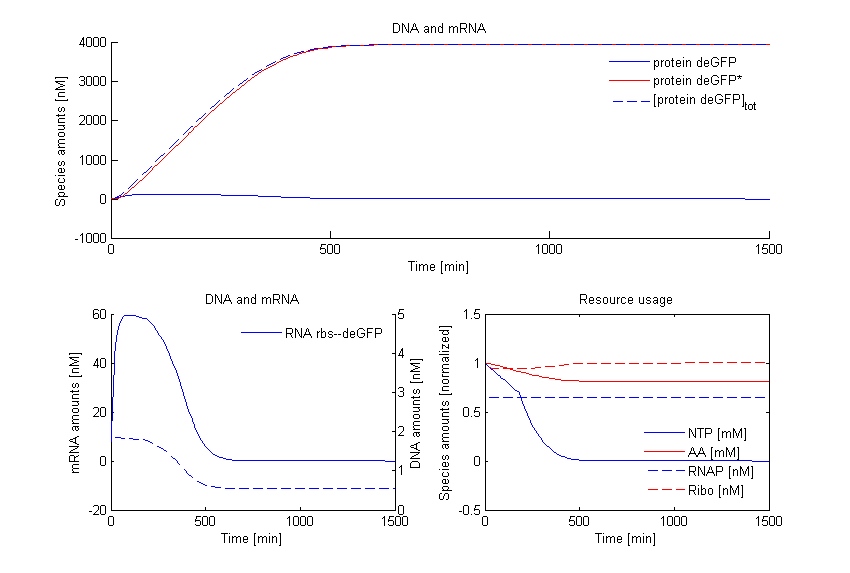
\includegraphics[width=\textwidth]{GeneExpressionPlotActuallyProducedByCode.png} 
		\caption{Gene Expression Output}
		\label{fig:geneexpr}
		\end{center}
		
		\end{figure}
		
%% NEGATIVE AUTOREG
	\section{Negative Autoregulation (\texttt{negautoreg})}
%%%% OVERVIEW	
		\subsection{Overview}
		Negative autoregulation refers to the repression of gene expression by a protein encoded by that very gene. In this code, we will show that dimerized tetR protein represses its own production, and thus leads to a relatively low steady state concentration. 
		\subsection{Code}
		Please work through the Gene Expression example above to get basic familiarity with the commands and their usage. This example is slightly more complex than \texttt{geneexpr}. We provide the entire code for this example below: \\
		
		\noindent \texttt{tube1 = txtl\_extract('E8');} \\
								\texttt{tube2 = txtl\_buffer('E8');} \\
								\texttt{tube3 = txtl\_newtube('circuit');} 
								\vspace*{1\baselineskip}
								
								\noindent \texttt{dna\_tetR = txtl\_add\_dna(tube3, 'thio-junk(500)-ptet(50)', 'rbs(20)', 'tetR(647)-lva(40)', 16, 'linear'); }\\
								\texttt{dna\_deGFP = txtl\_add\_dna(tube3, 'p70(50)', 'rbs(20)', 'deGFP(1000)', 16, 'linear');}\\
								\texttt{dna\_gamS = txtl\_add\_dna(tube3, 'p70(50)', 'rbs(20)', 'gamS(1000)', 1, 'plasmid');}
								\vspace*{1\baselineskip}
								
								\noindent \texttt{Mobj = txtl\_combine([tube1, tube2, tube3]);} 
								\vspace*{1\baselineskip}	
								
								\noindent \texttt{configsetObj = getconfigset(Mobj, 'active');}\\
								\texttt{set(configsetObj, 'StopTime', 8*60*60);}\\
								\texttt{[t\_ode, x\_ode, mObj, simData] = txtl\_runsim(Mobj, configsetObj);}
								\vspace*{1\baselineskip}
								
									 \begin{flushleft}
						 \texttt{\noindent dataGroups\{1,1\} = 'DNA and mRNA'; \\
						dataGroups\{1,2\} = \{'ALL\_DNA'\};\\ 
						dataGroups\{1,3\} = \{'b-','r-','b--','r--','y-','c-','g-','g--'\};\\}
						\vspace*{1\baselineskip}
						\texttt{\noindent dataGroups\{2,1\} = 'Gene Expression';\\
						dataGroups\{2,2\} = \{'protein tetR-lva-terminatordimer'\};;\\
						dataGroups\{2,3\} = \{'g-','b-','g--','b--','r--','b-.','c-','y--','m-','k-','r-'\};\\}
						\vspace*{1\baselineskip}
						\texttt{\noindent dataGroups\{3,1\} = 'Resource usage';\\}
						\vspace*{1\baselineskip}
						 \texttt{\noindent txtl\_plot(t\_ode,x\_ode,Mobj,dataGroups); \\} 
						 \end{flushleft}
		
		The important differences from the gene expression examples are that here we add 3 pieces of DNA into tube 3, two of which are linear. \\
		The tetR DNA uses a ptet promoter, which is repressed by the tetR protein dimer. Attached to the ptet promoter, there are two domains (thiosulfate 'thio' and junk DNA 'junk) which lower the rate of DNA degradation by the exonuclease RecBCD. The tetR DNA also shows an 'lva' tag, which attaches a amino acid sequence to the tetR protein and marks it for degradation by the protease ClpXP. In a futire version, all the 'lva' tags will be replaced by the 'ssrA' tags, although for the functioning of this toolbox, this name change is inconsequential. The reaction rate parameters for ClpXP's action are currently in the process of being determined. \\
		The second DNA, deGFP, is just like in the gene expression exampe, except that in this case it is mounted on a 'linear' DNA, and therefore can be degraded. \\ 
		The third DNA, gamS, is mounted onto a plasmid, and is thus safe from degradation. GamS helps to sequester the RecBCD exonuclease, providing protection tot the DNA. \\
		%Note that as opposed to the plotting function in the gene expression example, here we call txtl\_plot without the data groups input, and so the plotting function uses the defaults. 
		
		
		\subsection{Results}	
		
		\begin{figure}
		\begin{center}
		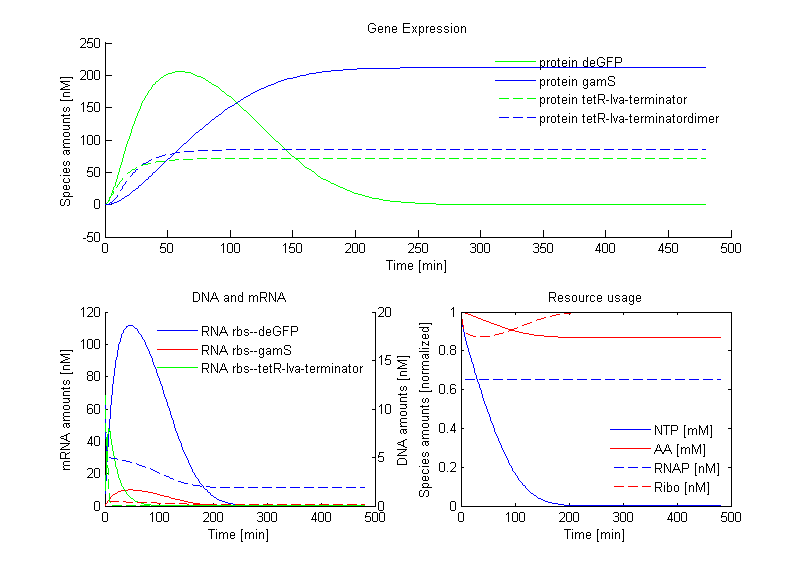
\includegraphics[width=\textwidth]{NegativeAutoregulationPlotActuallyProducedByCode.png} 
		\caption{Negative Autoregulation Output}
		\label{fig:negautoreg}
		\end{center}
		
		\end{figure}
		Figure \ref{fig:negautoreg} illustrates a number of features: expression of gamS, tetR and the tetR dimer, the respective mRNAs, and resources. The first thing to note is that expression levels in this example are an order of magnitude lower than in gene expression. There are two reasons for this: The use of 'linear' DNA, which means that RecBCD mediated DNA degradation is active, and the quick depletion of the RNA, due to the greater amount of RNA produced.  
		
	\section{Induction of Gene Expression using aTc (\texttt{induction})}
		\subsection{Overview}
		In this circuit, we explore the effect of varying levels of the inducer 'aTc' on the expression of a gene under the control of the tetR repressed ptet promoter. The expressed gene is precisely the tetR protein, leading to a negative autoregulation circuit as in the previous example. This DNA is loaded onto a plasmid DNA, and so no DNA degradation occurs. Figure \ref{fig:inductionSchematic} shows the circuit diagram for this example. Note that in the diagram, the deGFP and tetR are fused, while in the simulation, we only use the tetR gene, but we set its length to be 1200, comparable to the length of the tetR-deGFP fusion DNA. \\ 

		\begin{figure}
		\begin{center}
		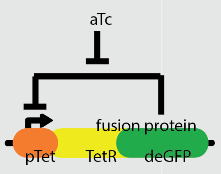
\includegraphics{negautoreg_induction schematic.png} 
		\caption{Schematic of the induction circuit'}
		\label{fig:inductionSchematic}
		\end{center}
		\end{figure}		
		
		 
		\subsection{Code}
		This code uses the \texttt{txtl\_addspecies} command to add increasing amounts of \texttt{'aTc'} to the model object, and executes the simulation. The Figure \ref{fig:induction} below plots the levels of tetR protein at different \texttt{'aTc'} concentrations. \\
		
		Set up tubes: \\
\noindent \texttt{tube1 = txtl\_extract('E6');} \\
\texttt{tube2 = txtl\_buffer('E6');} \\
\texttt{tube3 = txtl\_newtube('circuit');} 
\vspace*{1\baselineskip}
		
		Construct DNA and add to \texttt{tube3}: \\						
\noindent \texttt{dna\_tetR = txtl\_add\_dna(tube3, 'thio-junk(500)-ptet(50)', 'rbs(20)', 'tetR(1200)-lva(40)', 16, 'plasmid'); } \\
\texttt{dna\_gamS = txtl\_add\_dna(tube3, 'p70(50)', 'rbs(20)', 'gamS(1000)', 0, 'plasmid');}
\vspace*{1\baselineskip}
			
		Add protein gamS to the model. We used \texttt{txtl\_add\_dna} to set up its reactions. \\
		
		\noindent \texttt{gamS = txtl\_addspecies(tube3, 'protein gamS', 100);}
\vspace*{1\baselineskip}
				
		Define levels of \texttt{aTc} to use. \\						
\noindent \texttt{count = 1;}\\
% Do runs at different inducer levels
\texttt{levels = [0 2 5 10 20 40 100 300 1000];}\\
\texttt{colors = \{'r', 'b', 'g', 'c', 'm', 'y', 'k', 'r--', 'b--'\};}
\vspace*{1\baselineskip}
								
		Combine tubes: \\						
\noindent \texttt{Mobj = txtl\_combine([tube1, tube2, tube3]);}
\vspace*{1\baselineskip}
								
		Iteratively Simulate the model with different levels of aTc. \\						
\noindent \texttt{for atc = levels }\\
 \texttt{configsetObj = getconfigset(Mobj, 'active');}\\
  \texttt{set(configsetObj, 'StopTime', 6*60*60);  }\\
  \texttt{[t\_ode, x\_ode, Mobj, simData] = txtl\_runsim(Mobj, configsetObj); }
\vspace*{1\baselineskip}
								
\noindent \texttt{figure(2); hold on;}\\
  \texttt{itetR = findspecies(Mobj, 'protein tetR');}\\
  \texttt{plot(t\_ode, x\_ode(:, itetR), colors\{count\});}\\
  \texttt{labels{count} = [int2str(atc) ' nM aTc'];}
								\vspace*{1\baselineskip}
								
  % Add additional inducer for the next run
  \noindent \texttt{if count < size(levels,2)}\\
  \texttt{inducer = txtl\_addspecies(Mobj, 'aTc', levels(count+1)-levels(count));}\\
  \texttt{count = count + 1;}\\
  \texttt{end}\\
\texttt{end}
	\vspace*{1\baselineskip}
								
\noindent \texttt{title('Time Responses');}\\
\texttt{lgh = legend(labels, 'Location', 'Northwest');}\\
\texttt{legend(lgh, 'boxoff');}\\
\texttt{ylabel('Species amounts [nM]');}\\
\texttt{xlabel('Time [min]');}

		
		
		\subsection{Results}	
		\begin{figure}
		\begin{center}
		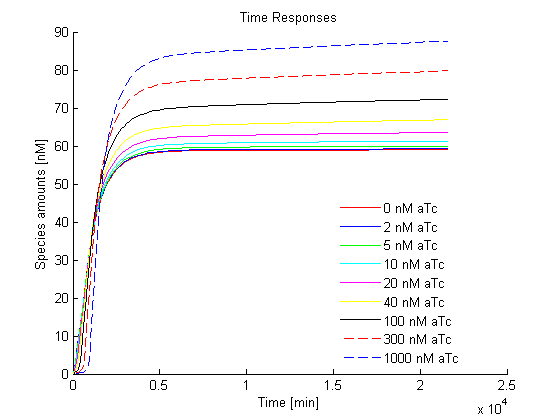
\includegraphics[width=\textwidth]{induction.png} 
		\caption{Induction of tetR expression due to aTc}
		\label{fig:induction}
		\end{center}
		
		\end{figure}
		Figure \ref{fig:induction} shows the concentrations of tetR. Note that this is not the standard plot generated in the previous two examples. We used the \texttt{findspecies} function to obtain the index of the species to plot (\texttt{[protein tetR]}) by using that index to access the relevant column of the data vector \texttt{x\_ode}. \\
		
		We note that as the \texttt{aTc} concentration is increased, the level of \texttt{tetR} in the system increases due to reduced repression of \texttt{ptet} by \texttt{protein tetRdimer}. 
		
%	\section{Incoherent Feedforward Loop (incoherent\_ff\_loop)}
%		\subsection{Overview}
%		\subsection{Code}
%		\subsection{Results}	

% \chapter{\textsc{Creating new circuits}}
	%\section{Creating Circuit Based on Library Components}
	
% \section{Creating a Library Component}
% 	\section{Creating a Parameter File}
\chapter{\textsc{Core Functionalities}} 
%% INTRODUCTION
	%\section{Introduction}
%	<Add a diagram showing the main species and reactions. The full list of reactions can be found in the appendix.>
%% USER COMMANDS	
	\section{User Commands}	
	Here we give details about the various functions you will be using in the modelling toolbox. 	

%%%% TXTL_EXTRACT	
		\subsection*{\texttt{txtl\_extract}}
			Set up a tube containing the TXTL 'Extract'. This is usually the first function to be called, and sets up various basic reaction rates, species and reactions. It takes the name of a configuration file containing parameter values as an input and returns a pointer to a Simbiology model object.  \\	
			\\
			The syntax and the usage of this function are summarized below, along with the species, reactions, parameters, and initial concentrations the function sets up:
			
			\begin{tabular}{p{2cm}|p{13cm}}
			Syntax & \texttt{tube = txtl\_extract(name)}\\ \hline
			Input & \texttt{name}: (string) name of extract \\ \hline
			Output & \texttt{tube}: pointer to Simbiology model object\\ \hline
			Usage & \texttt{tube1 = txtl\_extract('E6');}\\ \hline
			Species & RNAP, Ribo, $\sigma 28$ and $\sigma 70$, RecBCD, RNA-ase \\ \hline
			Reactions & Formation of RNAP70 and sequestration of RecBCD \\ \hline
			Parameters & Set-up reaction rates, AA and NTP models, and initial amounts defined in the \texttt{txtl\_reaction\_config} class. See \texttt{txtl\_reaction\_config} in \S 3.3 for more information. This function also sets-up the initial amounts for Ribosomes, RNAP,  $\sigma 28$ and $\sigma 70$. Their values can be found in the file, including the references they were extracted from. \\
			\end{tabular}
			
%%%% TXTL_BUFFER			
		\subsection*{\texttt{txtl\_buffer}}
		Set up a tube containing the TXTL 'Buffer'. This sets up the NTP and AA species, with initial concentrations from the supplied configuration file (same as the one used for the 'Extract'). \\
					
			\begin{tabular}{p{2cm}|p{13cm}}
			Syntax & \texttt{tube = txtl\_buffer(name)}\\ \hline
			Input & \texttt{name}: (string) name of buffer. \\ \hline
			Output & \texttt{tube}: pointer to Simbiology model object\\ \hline
			Usage & \texttt{tube2 = txtl\_buffer('E6');}\\ \hline
			Species & NTP and AA \\
			\end{tabular}

%%%% TXTL_NEWTUBE						
		\subsection*{\texttt{txtl\_newtube}}	
		Create a new model object ('tube') containing one compartment called 'contents'). \\	
			
			\begin{tabular}{p{2cm}|p{13cm}}
			Syntax & \texttt{tube = txtl\_newtube(name)}\\ \hline
			Input & \texttt{name}: (string) name of new tube. \\ \hline
			Output & \texttt{tube}: pointer to Simbiology model object\\ \hline
			Usage & \texttt{tube3 = txtl\_newtube('circuit');}\\
			\end{tabular}	

%%%% TXTL_ADD_DNA								
		\subsection*{\texttt{txtl\_add\_dna}}
			This function creates a piece of DNA that the user specifies, and sets up all the associated species and reaction objects, initial concentrations, and reaction rate parameters. The tube the DNA is placed in, the initial amount, and the type of DNA, 'linear' or 'plasmid', are specified by the user. The function returns a pointer to the DNA species object. \\ 
			\\
			This is summarized below:	
			
			\begin{tabular}{p{2cm}|p{13cm}}
			Syntax & \texttt{dna = txtl\_add\_dna(tube, prom\_spec, rbs\_spec, gene\_spec, dna\_amount, type)}\\ \hline
			Input &  \begin{itemize}
				\item \texttt{tube}: pointer to the model object to add the DNA to.
				\item \texttt{prom\_spec}: (string) string representing promoter. See below for details. 
				\item \texttt{rbs\_spec}: (string) ribosome binding site with optional length in Base Pairs.
				\item \texttt{gene\_spec}: (string) gene string. See below.
				\item \texttt{dna\_amount}: (double) amount of DNA to be added, in nM. This will be the \textbf{final} concentration in the experiment after the tubes have been combined. 
				\item \texttt{type}: (string) type of DNA: 'linear' or 'plasmid'. 
				\end{itemize} \\ \hline
			Output & \texttt{dna}: pointer to DNA object. \\ \hline
			Usage & \texttt{dna\_tetR = txtl\_add\_dna(tube3, 'thio-junk(500)-ptet(50)', 'rbs(20)', 'tetR(647)-lva(40)-terminator(100)', 16, 'linear');}\\ \hline
%			Species & {\color{red}<to be added later>}\\ \hline
%			Reactions & {\color{red}<to be added later>}\\ \hline
%			Parameters & {\color{red}<to be added later>}\\
			\end{tabular}	
			
			\vspace{1\baselineskip}
						
The \texttt{prom\_spec} is a string containing the name of the promoter to be used (this is a necessary argument, and needs the corresponding promoter file to be present in the MATLAB search path), with an optional length in base pairs. If the length is not specified, the default length specified in a \textsf{txtl\_param\_<promoterName>.csv} file is used. There are two other optional strings that can be specified: a \texttt{'thio'} and a \texttt{'junk(n)'}, where n is an optional integer value. The \texttt{'thio'} string tells the Toolbox that a thiosulfate group is present , and this confers protection to the DNA from degradation. As of this release, the amount of protection is arbitrarily set, and will be corrected once the relevant experiments and system ID are carried out. Similarly, junk DNA slows down the DNA degradation rate by an amount proportional to the length of this DNA added, with the constant of proportionality to be determined. As an example, a full specification of this string would look like: \texttt{'thio-junk(500)-ptet(50)'}. Note that only 'linear' DNA can be degraded. 'plasmid' DNA does not degrade in this toolbox. 

The \texttt{gene\_spec} string works similarly to the \texttt{prom\_spec} string. The name of the gene is required, and this must be associated with an existing protein file. Defaults work similarly as in \texttt{prom\_spec}, with a required component configuration file. The optional strings are: 'ssrA(n)' and 'terminator(n)', where ssRA is a degradation tag (length n) which marks the protein for degradation, and the terminator will have capabilities in future releases of the toolbox. 

Note: Generally, the lengths in BP are used to calculate transcription and translation rates. These lengths will have greater prevalence in the calculation of reaction rates in future versions of the toolbox. 

%%%% TXTL_COMBINE
		\subsection*{\texttt{txtl\_combine}}
				Combine the contents (species and reactions) of tubes to form a new tube. \\	
			
			\begin{tabular}{p{2cm}|p{13cm}}
			Syntax & \texttt{Mobj = txtl\_combine(tubelist, vollist)}\\ \hline
			Input & \texttt{tubelist} (vector of pointers) A list of tubes to combine together. \\ \hline
			Output & \texttt{Mobj}: pointer to the new tube.\\ \hline
			Usage & \texttt{Mobj = txtl\_combine([tube1, tube2, tube3]}\\
			\end{tabular}
				
%%%% TXTL_RUNSIM					
		\subsection*{\texttt{txtl\_runsim}} 
		
		Simulate model. \texttt{txtl\_runsim} is the main function to execute the MATLAB differential equation solvers to solve for the species concentration trajectories forward in time from a specified initial condition. It returns a vector array \texttt{t\_ode\_output} containing time points and a matrix array \texttt{x\_ode\_output} containing the corresponding species concentration values. \texttt{x\_ode\_output} is arranged such that each column corresponds to a species, and contains that species' concentrations at the time points corresponding to the points specified in \texttt{t\_ode\_output}. \\
		
		\begin{tabular}{p{2cm}|p{13cm}}
			Syntax & \texttt{[t\_ode\_output, x\_ode\_output, Mobj] = txtl\_runsim(modelObj, configsetObj)}\\
			& or \\
			& \texttt{[t\_ode\_output, x\_ode\_output, Mobj, simData\_output] = txtl\_runsim(modelObj, configsetObj, t\_ode\_input, x\_ode\_input, simData\_input)}\\ \hline
			Input &  \begin{itemize}
				\item \texttt{modelObj}: pointer to the model object to simulate. This is the Simbiology model object returned by \texttt{txtl\_combine}.
				\item \texttt{configsetObj}: pointer to the configuration set object to be used to configure the simulation properties like the simulation stopping time. See below for details. Also, see the matlab documentation for the Simbiology toolbox function \texttt{addconfigset}. 
				\item \texttt{t\_ode\_input}: optional vector array containing time point data from previous runs. See below for more information. 
				\item \texttt{x\_ode\_input}: optional matrix array containing species concentration trajectory data from previous runs. See below for more information.
				\item \texttt{simData\_input}: optional structure containing simulation data, such as names of species. See below.   
				\end{itemize} \\ \hline
			Output & \begin{itemize}
				\item \texttt{t\_ode\_output}: vector array containing time point data from this run, appended to data from previous runs, if any. 
				\item \texttt{x\_ode\_output}: matrix array containing species concentration trajectory data from this run, appended to data from previous runs, if any.
				\item \texttt{Mobj}: model object the simulation was run on. 
				\item \texttt{simData\_output}: optional structure containing simulation data, such as names of species. See below.   
				\end{itemize} \\ \hline
			Usage & \texttt{[t\_ode, x\_ode, Mobj, simData] = txtl\_runsim(Mobj, configsetObj);}\\
			\end{tabular}
			
			\vspace{1\baselineskip}
			When a Simbiology model is created, there is a default configuration set object associated with it, and we can use the \texttt{getconfigset} command to get a pointer to this object. This is illustrated below by using 'active' argument, since when the model object is created, the default configuration set is the active one. We can then set its properties like the end time we want our model to be simulated until: \\
\texttt{configsetObj = getconfigset(Mobj, 'active');} \\
\texttt{set(configsetObj, 'StopTime', 8*60*60)} \\

After which we can execute \texttt{txtl\_runsim}: \\
\texttt{[t\_ode, x\_ode, Mobj, simData] = txtl\_runsim(Mobj, configsetObj);} 
% the configsetObj,. in a future version of this documentation, incluse sensitivity and events, and a more complete documentation on the configuratin set object. 

\vspace{1\baselineskip}
A useful feature of \texttt{txtl\_runsim} is that is allows one to 'continue' a simulation from the end point of a previous run, with new species of more of existing species added before the simulation is continued. This models the situation when additional reagents like inducers or proteins are added to an experimental preparation after the experiment has commenced. This can be done as follows: \\

First call to \texttt{txt\_runsim} \\
\texttt{[t\_ode, x\_ode, Mobj, simData] = txtl\_runsim(Mobj, configsetObj);} \\

Execute other code, say, add some inducer: \\
\texttt{aTc = txtl\_addspecies(mObj, 'aTc', 50);}\\

Continue simulation:\\
\texttt{[t\_ode2, x\_ode2, Mobj, simData] = txtl\_runsim(Mobj, configsetObj, t\_ode, x\_ode, simData);} \\

The new arrays \texttt{t\_ode2, x\_ode2} contain the results of the first simulation appended to the results of the second simulation. Thus, one can simply plot these to view the results since the beginning of the first simulation. 


		\subsection*{\texttt{txtl\_plot}}
		Plotting command that simplifies the plotting of the evolution of the concentrations of the standard species: Proteins of interest, Resources, and DNA and RNA concentrations. \\
		
		\begin{tabular}{p{2cm}|p{13cm}}
			Syntax & \texttt{txtl\_plot(t\_ode, x\_ode, Mobj);}\\
			& or \\
			& \texttt{txtl\_plot(t\_ode, x\_ode, Mobj, dataGroups);}\\		 \hline
			Input &  \begin{itemize}
				\item \texttt{t\_ode}: vector array containing time point data. 
				\item \texttt{x\_ode}: matrix array, with each column containing data corresponding to the time evolution of the concentration of once species in the model. See \texttt{txtl\_runsim} for more details.  
				\item \texttt{Mobj}: pointer to the model object associated with the data to be plotted.
				\item \texttt{dataGroups}: these are optional cell arrays of strings which enable the user to customize what is plotted. We will provide documentation on these in a future version of this manual.  
				\end{itemize} \\ \hline
			Usage & \texttt{txtl\_plot(t\_ode, x\_ode, Mobj);}\\
			& where \texttt{t\_ode, x\_ode} and \texttt{Mobj} are the variables defined in the file. 
			\end{tabular}
		% add info on data groups soon. 
		
%		\subsection*{txtl\_plot\_gui}
		
		\subsection*{\texttt{txtl\_addspecies}}
			\texttt{txtl\_addspecies} allows the addition of any species directly to the model object. If this species is already present in the model, the function simply increases its concentration by the amount that is added. If the species is a protein and is not present in the model, then \texttt{txtl\_addspecies} adds the protein, and sets up all the associated species (dimers, complexes) and reactions (repression, induction, degradation, etc.). \\
			
			\begin{tabular}{p{2cm}|p{13cm}}
			Syntax & \texttt{simBioSpecies = txtl\_addspecies(tube, name, amount)}\\ \hline
			Input &  \begin{itemize}
				\item \texttt{tube}: pointer to the model object to add the species to.
				\item \texttt{name}: (string) name of the species to be added. See below for format of string.  
				\item \texttt{amount}: (double) amount, in nM, of the species to add or to increase existing species' concentration by. 
				\end{itemize} \\ \hline
			Output & \texttt{simBioSpecies}: pointer to the species object just added.\\ \hline
			Usage & \texttt{inducer = txtl\_addspecies(Mobj, 'aTc', 20);}\\
			\end{tabular} \\
			
			
			Note that \texttt{name} strings have the following format: \\
			
			\begin{tabular}{|p{2cm}|p{13cm}|}
			\hline
			Standard species & \texttt{'<name of specie>'}\\ 
			& Examples: \texttt{'aTc'},  \texttt{'IPTG'},  \texttt{'ClpXP'} \\ \hline
			Expressed proteins & \texttt{'protein <name of protein>'} \\
			& Examples: \texttt{'protein tetR'},  \texttt{'protein lacI'} \\ \hline
			\end{tabular}
			% are there other types of species that can be added?
					
					
		\subsection*{\texttt{txtl\_findspecies}}
			\texttt{txtl\_findspecies} is a useful function to find the column index of a given species in the matrix data array (\texttt{x\_ode}) returned by \texttt{txtl\_runsim}. This enables the user to access the trajectory of any species in the model. \\
			
			\begin{tabular}{p{2cm}|p{13cm}}
			Syntax & \texttt{indexlist = findspecies(Mobj, namelist)}\\ \hline
			Input &  \begin{itemize}
				\item \texttt{Mobj}: pointer to the model object get species indices from.
				\item \texttt{namelist}: (string or cell array) name of the species to be searched for, or a cell array of such strings.
				\end{itemize} \\ \hline
			Output & \texttt{indexlist}: (integer or vector of integers) index of the species in the list of species in the model object, and in the data array \texttt{x\_ode} returned by \texttt{txtl\_runsim}. The vector is returned when \texttt{namelist} is a cell array, and the entries of the vector correspond to the indices for the entires in \texttt{namelist}. \\ \hline
			Usage & \texttt{iGFP = findspecies(Mobj, 'protein deGFP*');}\\
			& \texttt{iRNAP28\_DNA\_complex = findspecies(Mobj,'RNAP28:DNA p28\_ptet-{}-rbs-{}-deGFP')}
			\end{tabular} \\
			
			We can use the output of this function to plot the trajectory of the species as follows: \\
		\texttt{iGFP = findspecies(Mobj, 'protein deGFP*');}\\
  		\texttt{plot(t\_ode, x\_ode(:, iGFP));}	\\
  		  		
		or use the index directly: \\	
		\texttt{plot(t\_ode\_,x\_ode(:,findspecies(Mobj,'DNA p28\_ptet-{}-rbs-{}-deGFP:protein tetRdimer')),'r')} \\
		
		Note: one can see a list of all the species in the model by running the command \texttt{speciesNames = get(Mobj.species, 'name')}, where \texttt{Mobj} is the model object. 

\chapter{\textsc{Appendix}}

	\section{Externally Specified Parameters}
		\subsection*{txtl\_reaction\_config (class)}
		The txtl\_reaction\_config class enables users to input custom reaction parameters for the TXTL extract into their model. This is done via a comma-separated-value (.csv) file. The parameters controlled by this class are given in the properties of this class. 
		\subsubsection*{List of Parameters}
			\begin{enumerate}
			\item \textsc{NTPmodel}: 
			There are two models for transcription that the toolbox can switch between, model 1 and 2. We recommend keeping this setting at model 2, since model 1 suffers from stiffness of the differential equations to be solved, and is primarily used for testing purposes. 
        	\item \textsc{AAmodel}: 
        	Similar to NTPmodel above, we recommend keeping this setting at 2. 
        	\item \textsc{Transcription\_Rate}:
        	Reaction rate for: \\
        	\begin{align}
        	& \mathrm{NTP:RNAP^{70}:DNA} \rightarrow \mathrm{DNA} + \mathrm{RNA} + \mathrm{RNAP} 
        	\end{align}
        	and is inversely proportional to the RNA length (sum of rbs length and gene length). 
        	
        	\item \textsc{Translation\_Rate}: Reaction rate for: \\
        	% '[AA:' Ribobound.Name '] -> ' rna.Name ' + ' protein.Name ' +  Ribo'
        	\begin{align}
        	& \mathrm{AA:Ribo:RNA}  \rightarrow \mathrm{Protein} + \mathrm{RNA} + \mathrm{Ribo}
        	\end{align}
        	and is inversely proportional to the gene length. 
        	\item \textsc{DNA\_RecBCD\_Forward and DNA\_RecBCD\_Reverse}:
        	Complex formation and dissociation rate between RecBCD enzyme and DNA.        	
        	\begin{align}
        	& \mathrm{DNA} + \mathrm{RecBCD}  \rightleftharpoons \mathrm{DNA:RecBCD}
        	\end{align}
        	
        	
        	\item \textsc{DNA\_RecBCD\_complex\_deg}: 
        	Degradation rate of RecBCD-DNA complex. 
        	\begin{align}
        	& \mathrm{DNA:RecBCD} \rightarrow  \mathrm{RecBCD} 
        	\end{align}
        	
        	\item \textsc{Protein\_ClpXP\_Forward and Protein\_ClpXP\_Reverse}: 
        	
        	Complex formation and dissociation rate between ClpXP enzyme and a protein tagged for degradation.
        	\begin{align}
        	& \mathrm{Protein} + \mathrm{ClpXP} \rightleftharpoons  \mathrm{Protein:ClpXP} 
        	\end{align}        	
        	\item \textsc{Protein\_ClpXP\_complex\_deg} 
        	Degradation rate of ClpXP-Protein complex.
        	\begin{align}
        	& \mathrm{Protein:ClpXP}  \rightarrow   \mathrm{ClpXP}
        	\end{align} 
        	\item \textsc{RNAP\_S70\_F and RNAP\_S70\_R}:
        	RNAP70 formation and dissociation rate.
        	\begin{align}
        	& \mathrm{RNAP} + \sigma^{70} \rightleftharpoons   \mathrm{RNAP^{70}}
        	\end{align}
        	\item \textsc{AA\_Forward and AA\_Reverse}:
        	Binding and dissociation of AA to Ribosome mRNA complex:
        	\begin{align}
        	& \mathrm{AA} + \mathrm{Ribo:RNA}  \rightleftharpoons   \mathrm{AA}:\mathrm{Ribo:RNA}
        	\end{align}
        	\item \textsc{Ribosome\_Binding\_F and Ribosome\_Binding\_R}: Binding and dissociation rated fro RNA-Ribosome complex:
        	\begin{align}
        	& \mathrm{Ribo} + \mathrm{RNA}  \rightleftharpoons   \mathrm{Ribo:RNA}
        	\end{align}
        	\item \textsc{RNA\_deg}: RNA degradation rate:
        	\begin{align}
        	& \mathrm{RNA} + \mathrm{RNAase}  \rightarrow   \mathrm{RNAase}
        	\end{align}
        	
        	\item \textsc{NTP\_Forward and NTP\_Reverse}:
        	Binding and dissociation of NTP to the RNAP70-DNA complex:
        	% [' RNAPbound '] + NTP <-> [NTP:' RNAPbound ']
        	\begin{align}
        	& \mathrm{NTP} + \mathrm{RNAP^{70}}:\mathrm{DNA}  \rightleftharpoons   \mathrm{NTP}:\mathrm{RNAP^{70}}:\mathrm{DNA}
        	\end{align}
			\end{enumerate}		
		\subsubsection*{Configuration file: \textsf{'E<n>\_config.csv'}}
		The configuration file associated with this class is used to define the contents of the tubes created by the \texttt{txtl\_extract} and \texttt{txtl\_buffer}. the integer <n> in the name of the file refers to the label of the buffer and extract in the TXTL experimental protocol. For instance, if we use extract \textsf{'E6'} and buffer \textsf{'B6'} in the experimental protocol for a circuit, we would create a configuration file named \textsf{'E6\_config.csv'}, which would encapsulate the features of the extract and the buffer. We could then use this file in the modelling toolbox as follows: \\
		
		\noindent \texttt{tube1 = txtl\_extract('E6');} \\
		\texttt{tube2 = txtl\_buffer('E6');} \\
		
Note that we do not define two separate configuration files for the buffer and extract. All the information needed is stored in one file. \\

		\begin{figure}
		\begin{center}
		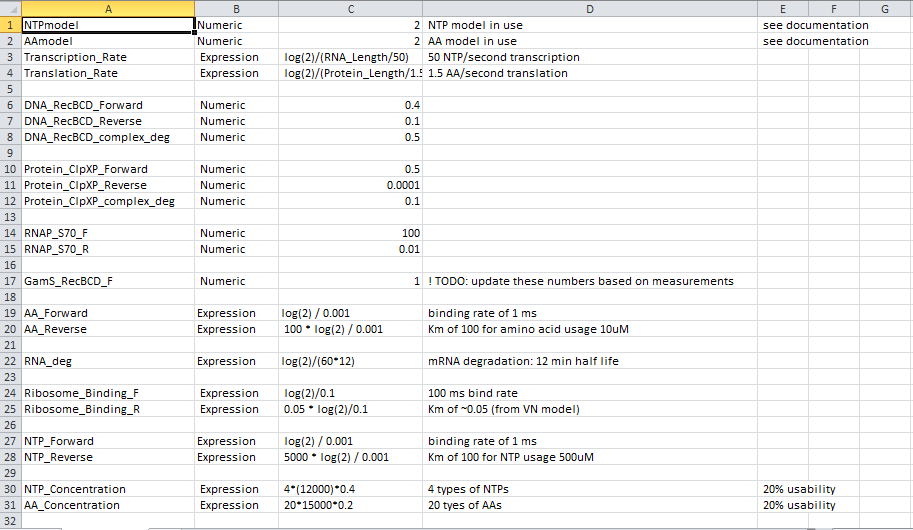
\includegraphics[width=\textwidth]{Config_E6_screenshot.png} 
		\caption{Screenshot of file 'E6\_config.csv'}
		\label{fig:reactionconfig}
		\end{center}
		\end{figure}

Figure \ref{fig:reactionconfig} shows a screenshot of the configuration file \textsf{'E6\_config.csv'} used in the \texttt{geneexpr} example. This file is a 'Comma Separated Value' file, and can be opened using Microsoft Excel. One can create custom configuration files by modifying the parameter values in this file, and saving it under a different name according to the naming convention defined above. 

		
		
		\subsection*{txtl\_component\_config (class)}	
		The txtl\_component\_config class enables users to input custom reaction parameters for the components they are using in their model. Components are found in the \textsf{components} directory in the main directory, and contain files that define proteins and promoters. The parameters present in the class and the corresponding configuration files are dependent on the components being used, but are highly analogous to the previous section. Editing of the configuration files is also carried out as above. 


	\section{List of Core Reactions}
	These reactions are currently those of Dan, and refer to the Toxin-Antitoxin System. We will modify them so that they correspond to the reactions in the TXTL toolbox. 
	
	
	\subsection{Basic}

\begin{align}
& \mathrm{RNAP} + \sigma^{70} \rightleftharpoons \mathrm{RNAP^{70}} \\
& P_{parDE}\textrm{--}rbs\textrm{--}deGFP + \mathrm{RNAP^{70}} \rightleftharpoons \mathrm{RNAP^{70}}\!:\!P_{parDE}\textrm{--}rbs\textrm{--}deGFP \\
& \mathrm{RNAP^{70}}\!:\!P_{parDE}\textrm{--}rbs\textrm{--}deGFP + \mathrm{NTP} \rightleftharpoons \nonumber \\ 
& \qquad \qquad \qquad \qquad \mathrm{NTP}\!:\!\mathrm{RNAP^{70}}\!:\!P_{parDE}\textrm{--}rbs\textrm{--}deGFP \\
& \mathrm{NTP}\!:\!\mathrm{RNAP^{70}}\!:\!P_{parDE}\textrm{--}rbs\textrm{--}deGFP \rightarrow \nonumber \\ 
& \qquad \qquad \qquad \qquad P_{parDE}\textrm{--}rbs\textrm{--}deGFP +  (rbs\textrm{--}deGFP)_m + \mathrm{RNAP^{70}} \\
\end{align}
	
	\subsection{Transcription}

\begin{align}
& \mathrm{RNAP} + \sigma^{70} \rightleftharpoons \mathrm{RNAP^{70}} \\
& P_{parDE}\textrm{--}rbs\textrm{--}deGFP + \mathrm{RNAP^{70}} \rightleftharpoons \mathrm{RNAP^{70}}\!:\!P_{parDE}\textrm{--}rbs\textrm{--}deGFP \\
& \mathrm{RNAP^{70}}\!:\!P_{parDE}\textrm{--}rbs\textrm{--}deGFP + \mathrm{NTP} \rightleftharpoons \nonumber \\ 
& \qquad \qquad \qquad \qquad \mathrm{NTP}\!:\!\mathrm{RNAP^{70}}\!:\!P_{parDE}\textrm{--}rbs\textrm{--}deGFP \\
& \mathrm{NTP}\!:\!\mathrm{RNAP^{70}}\!:\!P_{parDE}\textrm{--}rbs\textrm{--}deGFP \rightarrow \nonumber \\ 
& \qquad \qquad \qquad \qquad P_{parDE}\textrm{--}rbs\textrm{--}deGFP +  (rbs\textrm{--}deGFP)_m + \mathrm{RNAP^{70}} \\
& P_{70}\textrm{--}rbs\textrm{--}parD + \mathrm{RNAP^{70}} \rightleftharpoons \mathrm{RNAP^{70}}\!:\!P_{70}\textrm{--}rbs\textrm{--}parD \\
& \mathrm{RNAP^{70}}\!:\!P_{70}\textrm{--}rbs\textrm{--}parD + \mathrm{NTP} \rightleftharpoons \nonumber \\ 
& \qquad \qquad \qquad \qquad \mathrm{NTP}\!:\!\mathrm{RNAP^{70}}\!:\!P_{70}\textrm{--}rbs\textrm{--}parD \\
& \mathrm{NTP}\!:\!\mathrm{RNAP^{70}}\!:\!P_{70}\textrm{--}rbs\textrm{--}parD \rightarrow \nonumber \\ 
& \qquad \qquad \qquad \qquad P_{70}\textrm{--}rbs\textrm{--}parD +  (rbs\textrm{--}parD)_m + \mathrm{RNAP^{70}} \\
& P_{70}\textrm{--}rbs\textrm{--}parE + \mathrm{RNAP^{70}} \rightleftharpoons \mathrm{RNAP^{70}}\!:\!P_{70}\textrm{--}rbs\textrm{--}parE \\
& \mathrm{RNAP^{70}}\!:\!P_{70}\textrm{--}rbs\textrm{--}parE + \mathrm{NTP} \rightleftharpoons \nonumber \\ 
& \qquad \qquad \qquad \qquad \mathrm{NTP}\!:\!\mathrm{RNAP^{70}}\!:\!P_{70}\textrm{--}rbs\textrm{--}parE \\
& \mathrm{NTP}\!:\!\mathrm{RNAP^{70}}\!:\!P_{70}\textrm{--}rbs\textrm{--}parE \rightarrow \nonumber \\ 
& \qquad \qquad \qquad \qquad P_{70}\textrm{--}rbs\textrm{--}parE +  (rbs\textrm{--}parE)_m + \mathrm{RNAP^{70}}
\end{align}

\subsection{Translation}

\begin{align}
& \mathrm{R} + (rbs\textrm{--}deGFP)_m \rightleftharpoons \mathrm{R}\!:\!(rbs\textrm{--}deGFP)_m \\
& \mathrm{R}\!:\!(rbs\textrm{--}deGFP)_m + \mathrm{AA} \rightleftharpoons \mathrm{AA}\!:\!\mathrm{R}\!:\!(rbs\textrm{--}deGFP)_m \\
& \mathrm{AA}\!:\!\mathrm{R}\!:\!(rbs\textrm{--}deGFP)_m \rightarrow (rbs\textrm{--}deGFP)_m + \mathrm{deGFP} + \mathrm{R} \\
& \mathrm{R} + (rbs\textrm{--}parD)_m \rightleftharpoons \mathrm{R}\!:\!(rbs\textrm{--}parD)_m \\
& \mathrm{R}\!:\!(rbs\textrm{--}parD)_m + \mathrm{AA} \rightleftharpoons \mathrm{AA}\!:\!\mathrm{R}\!:\!(rbs\textrm{--}parD)_m \\
& \mathrm{AA}\!:\!\mathrm{R}\!:\!(rbs\textrm{--}parD)_m \rightarrow (rbs\textrm{--}parD)_m + \mathrm{D} + \mathrm{R} \\
& \mathrm{R} + (rbs\textrm{--}parE)_m \rightleftharpoons \mathrm{R}\!:\!(rbs\textrm{--}parE)_m \\
& \mathrm{R}\!:\!(rbs\textrm{--}parE)_m + \mathrm{AA} \rightleftharpoons \mathrm{AA}\!:\!\mathrm{R}\!:\!(rbs\textrm{--}parE)_m \\
& \mathrm{AA}\!:\!\mathrm{R}\!:\!(rbs\textrm{--}parE)_m \rightarrow (rbs\textrm{--}parE)_m + \mathrm{E} + \mathrm{R} 
\end{align}

\subsection{Degradation}

\begin{align}
& (rbs\textrm{--}deGFP)_m + \mathrm{RNase} \rightarrow  \mathrm{RNase} \\
& \mathrm{R}\!:\!(rbs\textrm{--}deGFP)_m + \mathrm{RNase} \rightarrow \mathrm{R} + \mathrm{RNase} \\
& \mathrm{AA}\!:\!\mathrm{R}\!:\!(rbs\textrm{--}deGFP)_m + \mathrm{RNase} \rightarrow \mathrm{AA} + \mathrm{R} + \mathrm{RNase} \\
& (rbs\textrm{--}parD)_m + \mathrm{RNase} \rightarrow  \mathrm{RNase} \\
& (rbs\textrm{--}parE)_m + \mathrm{RNase} \rightarrow  \mathrm{RNase} \\
& \mathrm{R}\!:\!(rbs\textrm{--}parD)_m + \mathrm{RNase} \rightarrow \mathrm{R} + \mathrm{RNase} \\
& \mathrm{R}\!:\!(rbs\textrm{--}parE)_m + \mathrm{RNase} \rightarrow \mathrm{R} + \mathrm{RNase} \\
& \mathrm{AA}\!:\!\mathrm{R}\!:\!(rbs\textrm{--}parD)_m + \mathrm{RNase} \rightarrow \mathrm{AA} + \mathrm{R} + \mathrm{RNase} \\
& \mathrm{AA}\!:\!\mathrm{R}\!:\!(rbs\textrm{--}parE)_m + \mathrm{RNase} \rightarrow \mathrm{AA} + \mathrm{R} + \mathrm{RNase}
\end{align}

\subsection{Protein complex association/dissociation}

\begin{align}
& \mathrm{D} + \mathrm{D} \rightleftharpoons \mathrm{D_2} \\
& \mathrm{E} + \mathrm{E} \rightleftharpoons \mathrm{E_2} \\
& \mathrm{D_2} + \mathrm{E_2} \rightleftharpoons \mathrm{D_2E_2} \\
& \mathrm{RecBCD} + \mathrm{GamS} \rightarrow \mathrm{RecBCD}\!:\!\mathrm{GamS} 
\end{align}

\subsection{Repression}

\begin{align}
& P_{parDE}\textrm{--}rbs\textrm{--}deGFP + \mathrm{D_2} \rightleftharpoons P_{parDE}\textrm{--}rbs\textrm{--}deGFP\!:\!\mathrm{D_2} \\
& P_{parDE}\textrm{--}rbs\textrm{--}deGFP + \mathrm{D_2E_2} \rightleftharpoons P_{parDE}\textrm{--}rbs\textrm{--}deGFP\!:\!\mathrm{D_2E_2}
\end{align}

\subsection{Other}

\begin{align}
& \mathrm{deGFP} \rightarrow \mathrm{deGFP^*}
\end{align}
	\section{List of Parameters}
	\begin{tabular}{|c|c|c|c|c|}
	\hline
	\textbf{Parameter} & \textbf{Description} & \textbf{Value} & \textbf{Source*} & \textbf{file} \\ \hline
	Transcription\_Rate & Rate of Transcription & $50 NTP/s$ & ? & \texttt{E6\_config.csv} \\ \hline
	Translation\_Rate & Rate of Translation & $1.5 AA/s$ & ? & \texttt{E6\_config.csv} \\ \hline
	DNA\_RecBCD\_Forward & Complex formation & $0.4 ?$ & ? & \texttt{E6\_config.csv} \\ \hline
	$\sim$ & Amount of RNAP & $100 nM$ & VN & \texttt{txtl\_extract.m} \\ \hline
	$\sim$ & Amount of $\sigma 70$ & $35 nM$ & VN & \texttt{txtl\_extract.m} \\ \hline
	$\sim$ & Amount of $\sigma 28$ & $20 nM$ & VN & \texttt{txtl\_extract.m} \\ \hline	
	$\sim$ & Amount of Ribosome & $1000 nM$ & $\sim$ & \texttt{txtl\_extract.m} \\ \hline
	$\sim$ & Amount of RecBCD & $100 nM$ & Amount to match RNAP & \texttt{txtl\_extract.m} \\ \hline
		$\sim$ & Amount of NTP & $100 nM$ & Amount to match RNAP & \texttt{txtl\_extract.m} \\ \hline
	\end{tabular}
	{\scriptsize * VN refers to publications by Vincent Noireaux (U. Minnesota).}

\end{document}
